\newpage

\section{Построение сети}

\subsection{Принципы построения производительных сетей}

Производительность системы определяется сочетанием её аппаратно- программных средств. Повышение производительности может быть достигнуто путем использования аппаратных средств, обладающих лучшими характеристиками производительности по сравнению с уже применяющимися.\par\bigskip

Повышение производительности сервера, следует производить в соответствии с предварительными расчетами “узких мест” – аналитическими расчетами, либо с помощью моделирования его работы. Эти расчеты показывают целесообразность увеличения производительности того или иного узла сервера - процессора, дисковой подсистемы. Аналогично для ЛВС можно определить, например, актуальность увеличения пропускной способности каналов связи.\par\bigskip

Производительность сервера зависит от наличия: 
\begin{itemize}
\item количества центральных процессоров;
\item шин PCI и их большой производительности;
\item большого объема памяти ОЗУ;
\item высокоскоростного дискового интерфейса;
\item организация дисковых подсистем с использованием RAID, обеспечивающих увеличение производительности.
\end{itemize}

\subsection{Принципы построения отказоустойчивых сетей}

Отказоустойчивость сети определяется двумя факторами:
\begin{itemize}
\item уровень избыточности сетевой инфраструктуры;
\item время восстановления сети, то есть время, необходимое для переключения потоков данных на работоспособные части сети в случае отказа ее части.
\end{itemize}\par\bigskip

При построении отказоустойчивой системы необходимо учесть следующее:
\begin{enumerate}
\item Архитектура сетевого оборудования:
    \begin{itemize}
    \item дублирование блоков питания;
    \item возможность "горячей" замены компонентов; 
    \item дублирование управляющего модуля; 
    \item ублирование коммутационной матрицы/шины.
    \end{itemize}
\item Дублирование соединений:
    \begin{itemize}
    \item использование нескольких дублирующих соединений; 
    \item не рекомендуется использовать протокол Spanning Tree, так как в сети появляется много неработающих (заблокированных) соединений, а время восстановления очень большое; 
    \item желательно использовать технологии Multi-Link Trunk (MLT) и Split-MLT (автоматическая балансировка потоков данных между всеми работоспособными соединениями; восстановление сети за доли секунды); 
    \item возможно внедрение протоколов балансировки нагрузки и дублирования на уровне маршрутизации;
    \item разнесение окончания каналов - окончание каналов на разных модулях ввода/вывода и/или на разных узлах для дополнительного дублирования;
    \item разнесение каналов - использование различных носителей и различных путей для критичных соединений;
    \end{itemize}
\item Высоконадежное сетевое оборудование - устройства с высоким временем наработки на отказ;
\item Отказоустойчивость сервера:
    \begin{itemize}
    \item использование технологии PCI Hot Plug замены отдельных узлов;
    \item многопроцессорные серверы;
    \item организация дисковых подсистем с использованием RAID, обеспечивающих увеличение надежности;
    \item дублирование дискового контроллера RAID;
    \item дублирование сетевых адаптеров;
    \item установка резервных вентиляторов для охлаждения процессора, ОЗУ, дисков, плат;
    \item организация резервного электропитания центрального процессора;
    \item резервирование источников питания;
    \item съемная плата кэш-памяти для диска со встроенной батареей;
    \item наличие заводского ВIOS (ПЗУ) и рабочего BIOS (ППЗУ).
    \end{itemize}
\end{enumerate}

\subsection{Расчёт вероятности безотказной работы дисковой подсистемы сервера}

Согласно ТЗ, необходимо определить вероятность безотказной работы дисковой подсистемы сервера, построенной на базе RAID-6, содержащей 3 базовых диска (без учета уровня RAID), при условии, что вероятность безотказной работы одного диска равна 0.6 и все диски одинаковые.\par\bigskip

RAID 6 имеет высокую степень надёжности — под контрольные суммы выделяется ёмкость 2 дисков, рассчитываются 2 суммы по разным алгоритмам. Обеспечивает работоспособность после одновременного выхода из строя двух дисков — защита от кратного отказа. То есть, массив выходит из строя только при отказе трёх и более дисков.\par\bigskip

Схема RAID-6 массива представлена на рисунке~\ref{pic:4_1_RAID-6}.

\begin{figure}[h]
\center{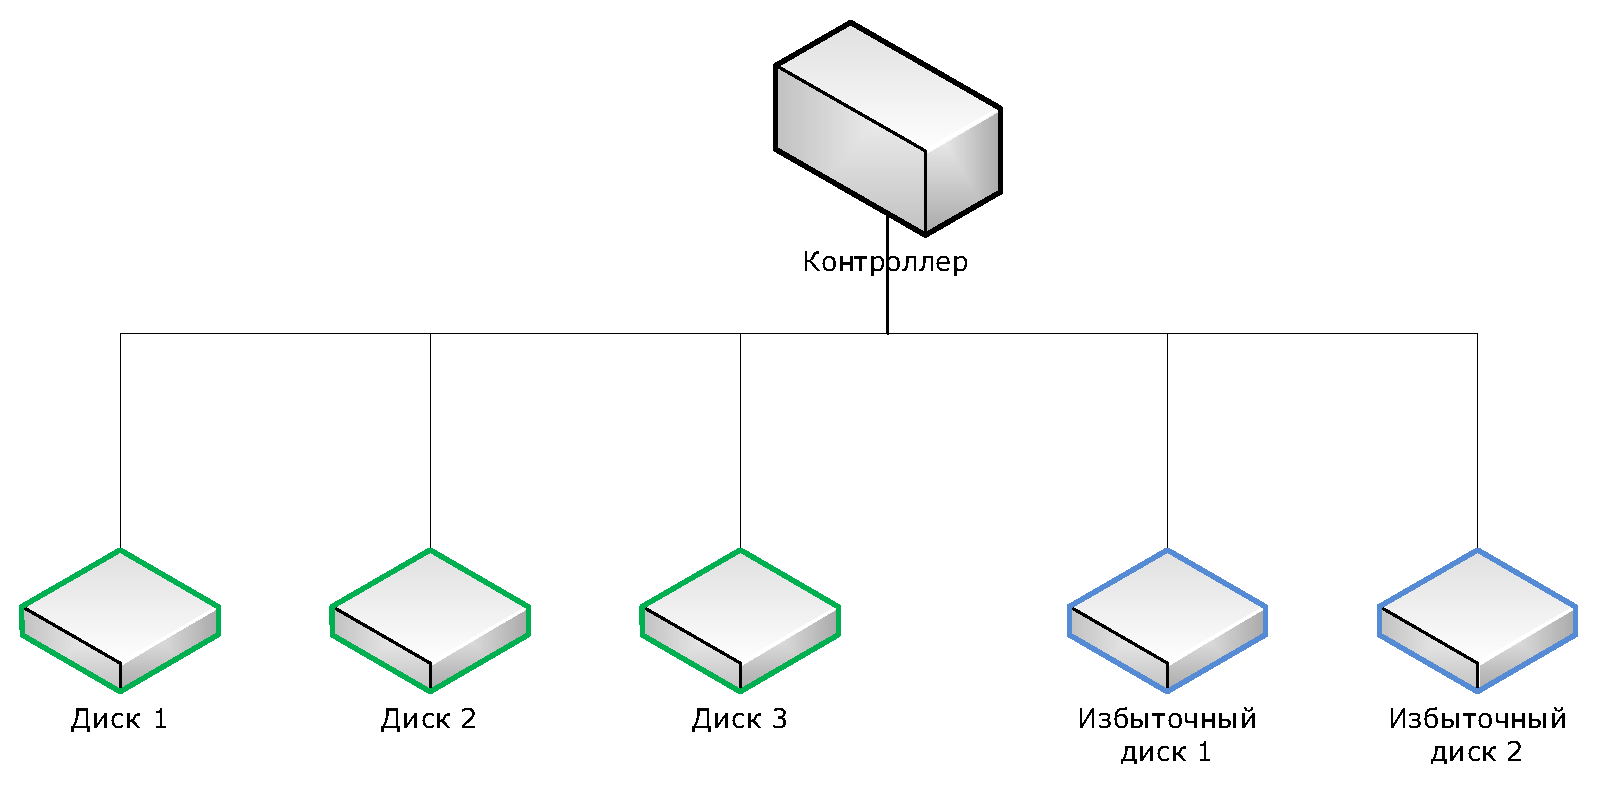
\includegraphics[width=0.7\linewidth]{pics/pic4_1_RAID-6.eps}}
\caption{Схема дискового массива RAID-6.}
\label{pic:4_1_RAID-6}
\end{figure}

Вероятность безотказной работы массива определяется по формуле:

$$P = 1 - \Bigr((1 - (1 - P_1)\cdot (1 - P_2))\cdot (1 - P_3)\Bigl)$$

Подставим значения вероятностей:
$$P = 1 - \Bigr(1 - (1 - 0.6)\cdot (1 - 0.6))\cdot (1 - 0.6)\Bigl)$$
$$P = 1 - 0.336 = 0.664$$

Таким образом, вероятность безотказной работы дисковой подсистемы сервера на базе RAID-6 равняется 0.664.

\subsection{Рекомендации по модернизации сети}

В центральном офисе и в первом филиале в сети используются устаревшие технологии: 10BASE-T и 10BASE-2. И если первую ещё можно модернизировать путём замены сетевых адаптеров и концентраторов с возможностью использования уже проложенного кабеля, то вторая потребует ещё и замены всего оборудования плюс демонтаж старого и прокладку нового кабеля.\par\bigskip

Если для работы фирмы достаточно текущей скорости передачи данных в сети и её пропускной способности, то не рекомендуется проводить модернизацию, так как это выльется в существенные финансовые и временные затраты.